\chapter{Variables In C}
When we want to store data to memory in assembly, we write to raw memory addresses. 
"Store this value to this address."
This obviously minimises the portability of our code as we would have to modify all of the memory addresses if we ported our code to a different system with a different memory architecture.
Instead of having to interface with memory directly, a more abstract language like C allows us to define and use \emph{variables}. 

A variable essentially allows you to give some memory a name and specify what operations can be done on that block of memory.
The amount of memory which the variable will be allocated and the operations which can be done to it are specified by the variable's \emph{data type}. 

One of the main advantages of using variables is that you do not need to specify or keep track of where your data will be stored in memory. The compiler\footnote{Technically it's the \emph{linker} which actually maps variable names to absolute memory addresses. Prior to linking, the memory addresses are all relative to segments.} keeps track of the mapping between the variable name and the memory addresses associated with that variable name.

\section{Types}
As mentioned earlier, the variable type specifies the amount of memory space which must be allocated for the variable and what operations can be done with or on that memory. The general format of a variable declaration is as follows.

\begin{lstlisting}[language=C]
type name = value;
\end{lstlisting}

We will now proceed to explore two of the most common types.

\subsection{Basic Types}
Basic types specify a block of memory which is treated as a simple number. While you do get basic types which support decimals, for most of our applications, the number will only be an integer. Much like how we had word, half-word or byte data types in assembly, we have similar number types in C.

C programmers frequently specify their types as either \texttt{char}, \texttt{int}, \texttt{short} or \texttt{long}. The problem with this is that the actual size of each of these types is not consistant across platforms. 
For example, the size of an \texttt{int} on your computer will be either 32 bits and 64 bits depending on which operating system you're running.

This ambiguity is an issue for us when working with microcontrollers. We often need to know exactly how much memory will be allocated to a variable. In order to specify the size of an int type exactly, we use the type definition \texttt{intx\_t} where \texttt{x} is either 8, 16, 32 or 64 and specifies the number of bits which must be allocated to that variable. The \texttt{\_t} indicates that it's a custom type which is defined in the \texttt{stdint.h} library. 

For example, the following definition will allocate 2 bytes of memory and call it \texttt{foo}.

\begin{lstlisting}[language=C]
int16_t foo;
\end{lstlisting}

The data held in the variable can either be treated as signed or unsigned data.
If a \texttt{u} is appended to the type the data should be treated as unsigned.
If no \texttt{u} is present the data should be treated as signed.

For example, in the following case \texttt{bar} is a signed number while \texttt{foo} is an unsigned number. 
\begin{lstlisting}[language=C]
uint32_t foo;
int32_t bar;
\end{lstlisting}

\subsection{Pointer Types}
We often want to deal with the memory addresses of variables or access specific addresses (such as in the case of interfacing with peripherals). For this, we can use pointer types. A pointer holds the address of some data. In other words, it point to some data.
The amount of data which is pointed to by the pointer is specified by the type. This means we need to specify two things when defining pointer types: we need to specify that the variable is a pointer type and we need to specify how much data is being pointed to.
We specify that it is a pointer using the asterisk. It is good practice to put the asterisk next to the variable name rather than next to the type.
For example, a pointer to 1 byte of data would be defined as follows\footnote{We specify the type again in brackets to do an explicit type cast. This is just to prevent a compiler warning by telling the compiler that we are intentionally (rather than accidentally) assigning a number to a pointer. Without the typecast, we would be assigning a basic type to a pointer type which would generate a warning.}.

\begin{lstlisting}[language=C]
int8_t *foo = (int8_t *)0x08001234;
\end{lstlisting}

Here, we are saying that the memory allocated to \texttt{foo} should point to the byte of data located at address.
Our address space runs from 0x0000 0000 to 0xFFFF FFFF which means that we need 4 bytes to store an address. Hence, no matter what the size of the data being pointed to is, a pointer type variable will always occupy 4 bytes in memory\footnote{This is architecture dependant though. A system which had a smaller or larger address space would require a different amount of data to be allocated for pointers.}.

Once we have a variable of type pointer, we are able to access the data being pointed to by the pointer with the dereference operator which is also an asterisk! This means that the asterisk has two possible meanings depending on context. If it's used during a variable declaration, it means the variable is of pointer type. If it is used on an existing variable of pointer type is means that we are accessing the data pointed to by the pointer, rather than accessing the pointer itself.

The following example shows defining a pointer, getting it to point to the address 0x2000 0550 and then modifying the data which is being pointed to.
\begin{lstlisting}[language=C]
uint32_t *bar;
bar = (uint32_t *)0x20000500;
*bar = 0xAABBCCDD;
\end{lstlisting}

The way arithmetic operations apply to pointers is different to the way arithmetic operations apply to basic types. With pointers, when you add or subtract values from the pointer, it actually adds or subtracts the value multiplied by the size of the data being pointed to. This can be thought of as causing the pointer to point to the next element of that type in memory, rather than just the next address.

A trivial example is shown below.
\begin{lstlisting}[language=C]
uint32_t  foo = 0x11223344;
uint32_t *bar = 0x11223344;
foo = foo - 1;   // foo now holds 0x11223343
bar = bar - 1;   // bar now holds 0x11223340
\end{lstlisting}

\subsection{Referencing}
We know that the address of variables is defined by the compiler. Suppose we want to ask the compiler what address it has assigned to a variable, how can we do that? The answer is by \emph{referencing} the variable. We've encountered dereferencing which essentially says "give me the data pointed to by this pointer." Referencing is the opposite process; it says "give me a pointer which points to this data." 

The reference operator is the ampersand operator. The datatype of a referenced variable is a pointer to the original type of the variable.
For example, the following defines a 8-bit integer \texttt{foo}, and then a pointer to an 8-bit integer \texttt{bar} which is then made to point to \texttt{foo}.

\begin{lstlisting}[language=C]
uint8_t foo = 0xAA;
uint8_t *bar;
bar = &foo;         // bar takes on the address of foo.
\end{lstlisting}

\section{Memory Allocation}
We now know that we can declare variables of different types which results in different amounts of memory being allocated to that variable. 
The question is, where does that memory get allocated?
Obviously, it must happen somewhere in RAM, as RAM is the block of memory which we use for general purpose data storage. 

The place is RAM which is used for the variable is determined by the storage duration or lifetime of the variable. 
There are two storage duration classes for variables: static and automatic. These will now be explored. 

\subsection{Static Variables}
Static variables are either allocated outside of functions (ie: global variables) or are allocated inside a function with the \texttt{static} qualifier keyword. 
The variable's lifespan is the entire duration of the program. That is, a spot in memory is allocated to that variable at compile time and that spot never changes or gets deallocated. No other variable will be allocated to that space.

Static variables are allocated memory at the \emph{start} of RAM. The block of memory which they live in is called the data segment. This is shown graphically in \autoref{fig:mem_allocation}.
Static variables are initialised to the value 0 unless you specify some other initial value.

\subsection{Automatic Variables}
We frequently only need a variable for some a short duration, such as when some function is called. When the function completes (returns) then that variable is no longer needed.
For this use-case, \emph{automatic} variables exist. 
These are variables which are only allocated a spot in memory when a function call happens and deallocated on return. 
Automatic variables are those which are defined inside a function without the \texttt{static} keyword. Any variable defined inside a function is called a local variable and is only visible within that function. This is as opposed to a global variable which is visible to all functions. 
The great advantage of automatic variables is that by only occupying memory for a short time we are able to make more efficient use of memory. 

Where do automatic variables get allocated in memory? Well, they need to be somewhere that easily the dynamic allocation and deallocation of memory. This is exactly that the stack does! When you \texttt{PUSH} a value to the stack it allocates some memory. When you \texttt{POP} a value it deallocates space on the stack. As such, the stack is used for automatic variables. Where the stack is and the direction which it grows in is shown in \autoref{fig:mem_allocation}.

\begin{figure}
    \centering
    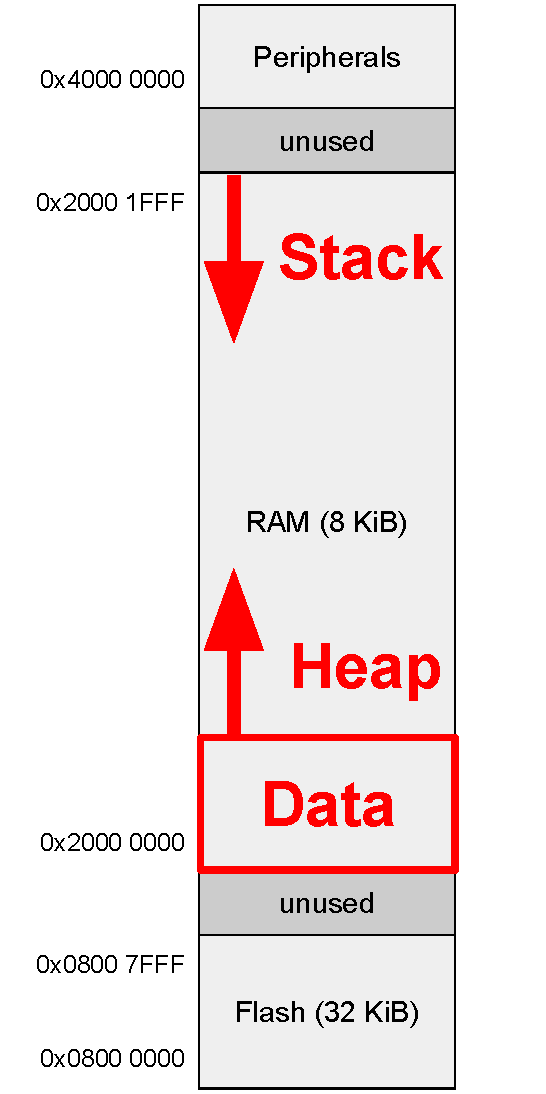
\includegraphics[scale=1]{./week8/mem_allocation.pdf}
    \caption{Layout of different variable blocks in memory. Note how data is fixed at compile time while stack and heap grow dynamically}
    \label{fig:mem_allocation}
\end{figure}

\subsection{Code Implementation}
The following is a simple example showing where and how different storage class variables are defined.

\begin{lstlisting}[language=C]
int8_t foo;                 // global static variable. 
void someFunction(void) {
    uin32_t bar;            // local automatic variable
    static int16_t baz;     // local static variable
}
\end{lstlisting}


\section{Arrays}
An array is a group of 1\footnote{As per C99 you can have zero-length array or flexible length arrays.} or more elements, each being of the same data type.
The array occupies an amount of memory equal to the sum of the memory required for each element. An array should be define in one of two different ways:
\begin{enumerate}
    \item Specifying the value for each element as an initialiser. In this case you do not need to specify the size of the array as it will be calculated by the compiler by counting the number if element values supplied.
    \item By specifying the size of the array and no initial values. Here the memory is allocated but no values is set for each element. If the array is a static variable, each element will be initialised to 0 by the startup code. If the array is an automatic variable each element will just be garbage by default. 
\end{enumerate}

An example of both of these ways is demonstrated below.


\begin{lstlisting}[language=C]
// The compiler allocates 5 bytes sets each to the specified value
int8_t foo[] = {0xAA, 0x42, 0x69, 0x55, 0xF0};

// The compiler allocates 15 words and leaves values as default
uint32_t bar[15];
\end{lstlisting}

The variable name (in the above example \texttt{foo} or \texttt{bar}) of an array type behaves in much the same way as if it were the address of element 0 of the array. 
This means firstly that you cannot write to the variable name, as it makes no sense to modify the address of element 0 after it has already been defined. 
Should you wish to access the element, you should first \emph{dereference} the variable which will give you access to the data. 
Should you wish to access element 1, you should add 1 to the address of element 0 and then deference that. 
This will always work independent of the size of the elements of the array due to arithmetic operations applied to pointer types working in multiplies of the size of the data being pointed to by the pointer, as discussed earlier.

